\chapter{Системийн шаардлага}

Уг бүлэг нь системийн хэрэглэгчийн зүгээс тавигдах шаардлагыг тодорхойлж, тухайн гаргасан шаардлагууд дээрээ үндэслэн UX судалгаа хийсэн талаарх гарах ба хэрэглэгч суурьтай интерфейс дизайн гаргахад тулгарсан асуудлуудыг товч дурдлаа.

\section{Шаардлагын шинжилгээ}

\subsection{Хэрэглэгчид}

Интернет сүлжээ ашиглан мэдээлэл авдаг, бусадтай хуваалцдаг бүх төрлийн хэрэглэгчид

\subsection{Функционал шаардлагууд}

\begin{table}[h]
	\centering
	\caption{Функциональ шаардлага}
	\begin{tabular}{ |p{2cm}|p{13cm}| }
	\hline
	ФШ 101 &  Веб нь бусад веб холбоосуудыг дангаар нь болон бүлэглэж оруулах боломжтой байх \\ \hline
	ФШ 102 &  Нийт хэрэглэгчдийн оруулсан веб холбоосууд, хэрэглэгчдийн мэдээллээс түлхүүр үгээр хайлт хийх боломжтой байх \\ \hline
	ФШ 103 &  Хэрэглэгч бүлэглэж оруулсан холбоосуудаа бусад хүмүүстэй хуваалцах боломжтой байх \\ \hline
	ФШ 104 &  Хэрэглэгч платформ дээрх дурын хүнээ дагах, түүний оруулсан веб холбоосуудыг харах боломжтой байх \\ \hline
	ФШ 105 &  Бусад хүмүүсийн оруулсан веб холбоосууд дээр хэрэглэгч үнэлгээ өгдөг боломжтой байх \\ \hline
	ФШ 106 &  Веб нь хэрэглэгчийн дагасан сэдвийн дагуу холбоосуудыг харуулдаг байх \\  \hline
	ФШ 107 &  Веб нь хэрэглэгч бүртгэх боломжтой байх \\ \hline
\end{tabular}
\end{table}

\subsection{Функционал бус шаардлагууд}

	\begin{table}[h]
		\centering
		\caption{Функциональ бус шаардлага}
		\begin{tabular}{ |p{2cm}|p{13cm}| }
		\hline
		ФБШ 101 &  Веб нь хэрэглэгч ашиглахад хялбар интерфейстэй байх \\ \hline
		ФБШ 102 &  Интерфейс дизайн нь түлхүү цагаан болон брэнд өнгийг хадгалсан шинэлэг дизайнтай байх \\ \hline
		ФБШ 103 &  Веб дээр нийтлэл оруулах үед бусад веб холбоосуудын Open Graph мэдээллийг 500 миллсекундэд багтаан авдаг байх \\ \hline
		ФБШ 104 &  Веб нь бүхий л төрлийн төхөөрөмжүүд дээр интерфейсийн алдаагүй ажиллах Responsive бүтэцтэй байх \\ \hline
		ФБШ 105 &  Веб холбоос оруулах үед дээд тал нь хоёр hashtag ашигладаг байх \\ \hline
		ФБШ 106 &  Хэрэглэгч хэдэн ч удаа веб холбоос оруулах боломжтой байх \\  \hline
	\end{tabular}
	\end{table}

\section{UX судалгаа}

Хэрэглэгч суурьтай дизайн гаргахад хамгийн чухал зүйл бол хэрэглэгчээ танин тэдгээрээс судалгаа авах, гаргасан үр дүнгээ ашиглан дизайнаа хөгжүүлэх, тодорхой тооны хэрэглэгчээр туршиулж сайжруулах үе шат юм. Миний хувьд эхлээд хэрэглэгчээ тодорхойлж, тус бүрийн Use Case-г гарган түүн дээ зориулан Wireframe хувилбар гаргасан. 

\pagebreak
\subsection{User Personas}

\subsubsection{Persona 1 - Болорчулуун}

\begin{figure}[h]
	\centering
	
\includegraphics[width=15cm]{images/persona1-bolorchuluun.png}
	\caption{Persona 1 - Болорчулууны мэдээлэл}
	\label{fig:persona1}
\end{figure}

\textbf{Use Case}

\begin{itemize}
	\item Өглөө ажил дээрээ эхний 20 минут мэргэжилтэйгээ холбоотой нийтлэлүүд унших дуртай
	\item Веб хөтөч дээрээ таалагдсан эсвэл дараа нь унших ёстой холбоосуудаа bookmark хийж хадгалж авдаг боловч зөвхөн ажлын компьютер дээр л тэдгээр холбоос маань хадгалагддаг. Өөр рүүгээ веб холбоосоо цуглуулж явуулахаас залхуу хүрдэг
\end{itemize}

\subsubsection{Persona 2 - Шүрэнцэцэгийн мэдээлэл}

\begin{figure}[h]
	\centering
	
\includegraphics[width=15cm]{images/persona2-shurentsetseg.png}
	\caption{Persona 2 - Шүрэнцэцэг}
	\label{fig:persona1}
\end{figure}

\textbf{Use Case}

\begin{itemize}
	\item Миний хувьд мэдээгээ бэлтгэхдээ дийлэнхдээ интернет дэх эх сурвалжуудаас бэлтгэдэг. Нэг асуудал байдаг маань эх сурвалж авдаг хэдхэн вэбсайт дунд л эргэлдэж байгаа.
	\item Олсон мэдээллүүдээ хамт ажиллаж буй хүмүүс рүүгээ явуулахдаа Telegram ашиглан нэг нэгээр нь хуулж тавин явуулдаг. Хүн болгон руу ингэж явуулах нь надад төвөгтэй байдаг
\end{itemize}

\subsection{Гаргасан интерфейс загварын эхний хувилбар}

Уг хэсэг дээр хэрэглэгчдийн Use Case, Empathy загвар дээр тулгуурлаж Wireframe болон High Fidelity түвшний интерфейс загвар гаргасан. Жишээ зургууд оруулав

\begin{figure}[h]
	\centering
	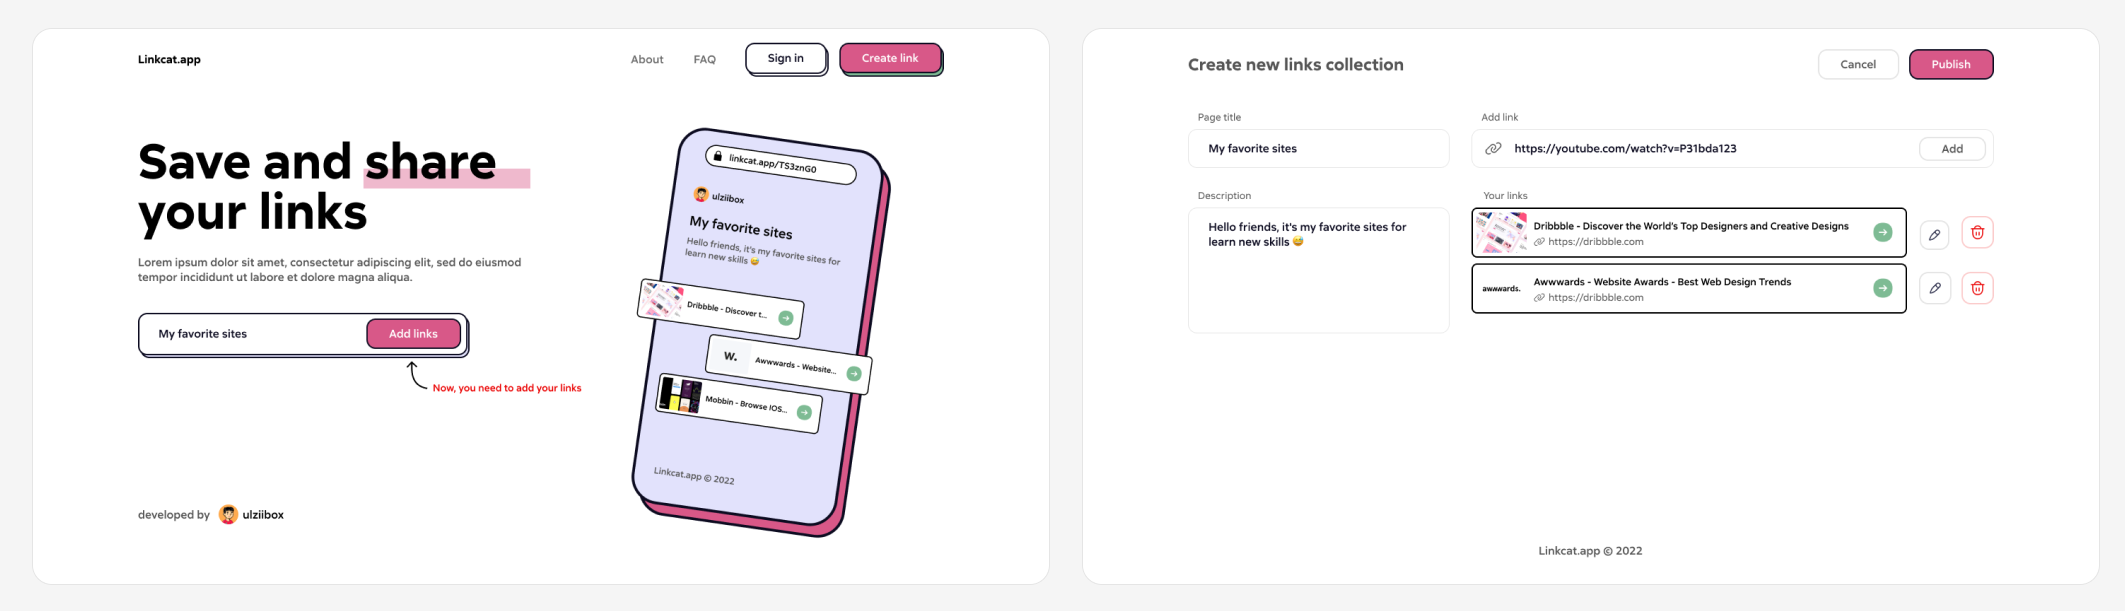
\includegraphics[width=15cm]{images/01-interface.png}
	\caption{Нүүр хуудас болон веб холбоос оруулах flow}
	\label{fig:interface1}
\end{figure}

\begin{figure}[h]
	\centering
	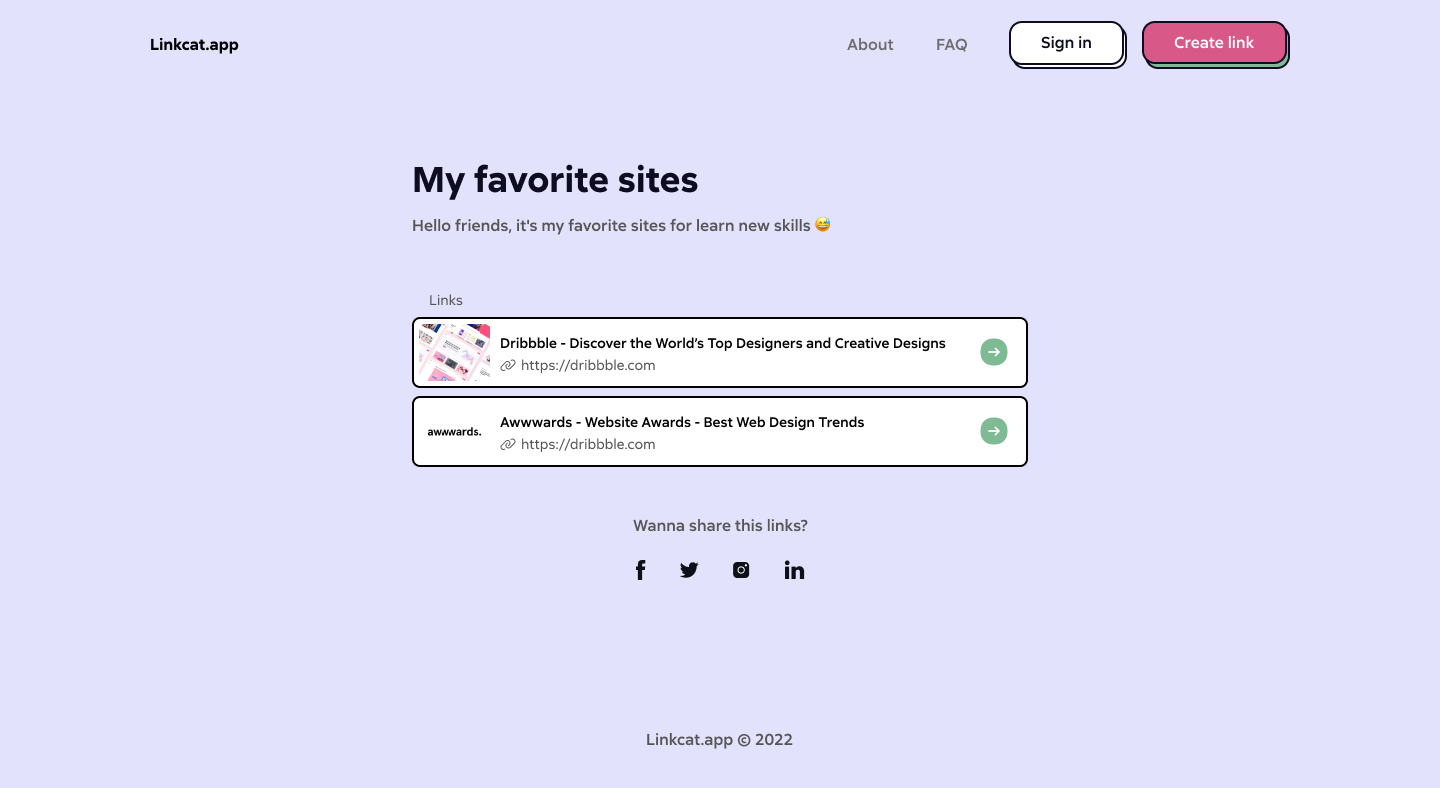
\includegraphics[width=15cm]{images/03-interface-page.png}
	\caption{Оруулсан веб холбоосуудыг бусад хэрэглэгчид харах хуудас}
	\label{fig:interface1}
\end{figure}
\pagebreak

\subsection{Usability туршилт}

Гаргасан интерфейс загваруудаа хооронд нь холбон Prototype түвшинд үндсэн үйлдлүүдээ хэрэглэгчээр туршуулж үзээд дараах дүгнэлтүүдэд хүрсэн. Үүнд

\begin{itemize}
	\item UI загвар нь тоглоом шиг өнгө төрхтэй байгааг сайжруулах
	\item Бусад хүмүүсийн оруулсан холбоосуудыг нэг дор харахыг хүссэн
	\item Зарим Use Case-үүдийн шаардлагыг хангаагүй
\end{itemize}

Иймд дараагийн бүлгийн \textbf{Хэрэглэгчийн интерфейс дизайн} хэсэгт гарах загварыг эцэслэн гаргасан болно.
